\hypertarget{a00365}{}\section{D\+S\+H Guide}
\label{a00365}\index{D\+S\+H Guide@{D\+S\+H Guide}}
How to test basic functionality of A\+A\+X plug-\/ins using D\+S\+H test tool. 

\hypertarget{a00365_dsh_guide_contents}{}\subsection{Contents}\label{a00365_dsh_guide_contents}
\begin{DoxyItemize}
\item \hyperlink{a00365_dsh_guide_00_what_is_dsh_and_how_it_works}{What is D\+S\+H and how it works} \item \hyperlink{a00365_dsh_guide_01_basic_set_of_commands_of_dae_dish}{Basic set of commands of the D\+A\+E dish} \item \hyperlink{a00365_dsh_guide_02_basic_plugin_tests}{Basic plug-\/in tests} \item \hyperlink{a00365_dsh_guide_03_debugging_and_tracing}{Debugging and tracing in D\+S\+H} \item \hyperlink{a00365_dsh_guide_04_scripting_interface_and_batch_profiling}{Scripting interface and batch profiling}\end{DoxyItemize}
 \hypertarget{a00365_dsh_guide_00_what_is_dsh_and_how_it_works}{}\subsection{What is D\+S\+H and how it works}\label{a00365_dsh_guide_00_what_is_dsh_and_how_it_works}
 Digi\+Shell is a software tool that provides a general framework for running tests on Avid audio hardware. As a command-\/line application, Digi\+Shell may be driven as part of a standard, automated test suite for maximum test coverage. D\+S\+H supports loading all types of A\+A\+X plug-\/ins except A\+S, and is especially useful when running performance and cancellation tests of A\+A\+X-\/\+T\+I types. Digi\+Shell is included in Pro Tools Development Builds as dsh.\+exe (Windows) or as dsh in the Command\+Line\+Tools directory (Mac).

After it is launched, Digi\+Shell waits for a command name and parameters to be entered via stdin; command results are output via stdout. Digi\+Shell parses its input as command name, followed by a single space, and then command parameters. The command parameters are expected to be a yaml-\/encoded string. Here are two examples of strings in compact (single-\/line) yaml format\+: 
\begin{DoxyItemize}
\item A hash containing lists in compact yaml syntax  {\ttfamily \{ key1\+: \mbox{[}val1, val2\mbox{]}, key2\+: \mbox{[}val3, val4\mbox{]} \}} ~\newline
  
\item A list of two lists  {\ttfamily \mbox{[}\mbox{[}P\+I\+O, 0, 1\mbox{]}, \mbox{[}D\+S\+P, 1, 1\mbox{]}\mbox{]}} 


\end{DoxyItemize}

 \hypertarget{a00365_dsh_guide_01_basic_set_of_commands_of_dae_dish}{}\subsection{Basic set of commands of the D\+A\+E dish}\label{a00365_dsh_guide_01_basic_set_of_commands_of_dae_dish}
 Digi\+Shell has built-\/in commands for getting help, creating a Digi\+Trace configuration and loading Digi\+Shell modules known as \char`\"{}dishes\char`\"{}. One can see the command list by running the help command without any parameters. Passing a command name as a single string parameter to the help command will give a more detailed command description.

The default installation of Digi\+Shell includes a few dishes, including the D\+A\+E dish. This dish loads the A\+A\+E audio engine and can be used for loading and testing basic functionality of plug-\/ins. The D\+A\+E dish can also be used to load a plug-\/in for basic debugging purposes, and provides a ligher-\/weight debugging environment than the full Pro Tools application.

Another dish supplied with D\+S\+H, the aaxh dish, provides a lower-\/level hosting environment for \hyperlink{a00288}{A\+A\+X} plug-\/ins. This dish loads a dedicated \hyperlink{a00288}{A\+A\+X} host component without audio routing logic or other audio engine responsibilities. In this guide we will focus on loading and running plug-\/ins using the D\+A\+E dish, but we encourage you to also explore the commands available in the aaxh dish and to learn how to exercise your plug-\/ins in that environment.

\hypertarget{a00365_subsection__loading_plugins}{}\subsubsection{Loading plug-\/ins in D\+S\+H}\label{a00365_subsection__loading_plugins}
 The following commands can be used to load and configure the D\+A\+E dish\+: 
\begin{DoxyItemize}
\item {\ttfamily load\+\_\+dish D\+A\+E}  Loads the D\+A\+E dish ~\newline
  
\item {\ttfamily init\+\_\+dae 48000}  This command is optional. It configures A\+A\+E to work at a specific sample rate. By default it will work at 44100 Hz.  
\end{DoxyItemize}

Loading the D\+A\+E dish into the Digi\+Shell environment with the built-\/in {\ttfamily load\+\_\+dish} command will extend the set of available commands. Amoung them there is a {\ttfamily run} command. The {\ttfamily run} command can be used in two ways\+:


\begin{DoxyItemize}
\item Execute with no arguments\+: List all plug-\/in configurations which are available to A\+A\+E  
\item Execute with arguments specifying a particular plug-\/in configuration\+: Load a plug-\/in instance using the specified configuration  
\end{DoxyItemize}

You can also search for the id and spec of the specific plug-\/in with the {\ttfamily findpi} command, which takes a plug-\/in\textquotesingle{}s name or part of it as an argument, and then searches through the whole list of available plug-\/ins using this pattern.

 Figure 1\+: D\+S\+H command for loading plug-\/ins.

If the plug-\/ins was instantiated successfully, then D\+S\+H will list all its parameters, just like on the screenshot. If instantiation fails, then D\+S\+H in most cases will output the error code, although it is not always obvoius what this error code means. Here is the list or possible reasons of some failures\+: 
\begin{DoxyItemize}
\item -\/9060 failed to load D\+S\+P Hybrid plug-\/in ~\newline
  
\item -\/14140 I\+O interface is not connected ~\newline
  
\item -\/7050 not enough resources for instantiating plugin ~\newline
  
\item -\/14378 plug-\/in exceeded memory limits ~\newline
  
\item -\/14003 something is wrong with your H\+D\+X card ~\newline
  
\end{DoxyItemize}

-\/30xxx errors are dynamically-\/generated and can indicate different failures. Failures due to plug-\/ins exceeding the cycle limit of the D\+S\+P C\+P\+U will often appear as -\/30xxx errors. See \hyperlink{a00362_subsection__30xxx_dynamic_error_codes}{-\/30xxx\+: Dynamically-\/generated error codes} in the \hyperlink{a00362}{T\+I Guide} for more information.

\begin{DoxyNote}{Note}
{\ttfamily run} command works for Native and D\+S\+P plug-\/ins, but not for the Audio Suite ones. Also it will fail for D\+S\+P Hybrid plug-\/ins. To be able to instantiate them, one should run {\ttfamily acquiredeck} command.
\end{DoxyNote}
There are several D\+A\+E dish commands for operating with plug-\/ins\textquotesingle{} instances\+: 
\begin{DoxyItemize}
\item {\ttfamily getcurrentinstance} Returns the index of the current instance. The counting strarts from 0 for the first instance that has been instantiated, and increments by one for every next instance. ~\newline
  
\item {\ttfamily getinstanceproperties} Returns the effect name for the Native plug-\/ins, and much more detailed info for the D\+S\+P instances.  
\item {\ttfamily setcurrentinstance} Sets the instance with the given index as the current instance.  
\end{DoxyItemize}

\hypertarget{a00365_subsection__working_with_hdx_card_from_dsh}{}\subsubsection{Working with H\+D\+X card from D\+S\+H}\label{a00365_subsection__working_with_hdx_card_from_dsh}
 One of the benefits of the D\+A\+E dish in Digi\+Shell is that it has direct access to the shell environment that loads D\+S\+P plug-\/ins. The included facilities for retrieving load error information from the D\+S\+P manager can be very helpful for debugging D\+S\+P plug-\/in load failures. For example, you can use the following D\+A\+E dish commands to determine what resource requirement is preventing additional instances from loading onto a single D\+S\+P\+: 
\begin{DoxyEnumerate}
\item {\ttfamily reservetidsp all} Reserves all unused D\+S\+Ps in the system  
\item {\ttfamily unreservetidsp 0} Frees the first D\+S\+P for plug-\/in allocation  
\item {\ttfamily getlastdsploaderror} Retrieve the text of the error that was generated when the final Effect instance attempted to load  
\item {\ttfamily getdspinfo 0} Returns detailed info about the D\+S\+P chip with the given index. By executing this command you can figure out whether particular chip is in use currently, which plug-\/ins are instantiated there, how many resources they consume and how many resources are still available. ~\newline
   Figure 2\+: Info about the D\+S\+P chip with the given index.  
\end{DoxyEnumerate}

\hypertarget{a00365_subsection__dsh_tips}{}\subsubsection{D\+A\+E dish tips}\label{a00365_subsection__dsh_tips}
 
\begin{DoxyItemize}
\item With the standard configuration, the system\textquotesingle{}s \hyperlink{a00288}{A\+A\+X} plug-\/ins folder will be used by D\+S\+H and D\+T\+T. To override this, create a folder named \char`\"{}\+Plug-\/\+Ins\char`\"{} next to the D\+T\+T and Command\+Line\+Tools directories. While that directory exists, A\+A\+E will only scan the plug-\/ins in the new Plug-\/\+Ins folder.  
\end{DoxyItemize}



 \hypertarget{a00365_dsh_guide_02_basic_plugin_tests}{}\subsection{Basic plug-\/in tests}\label{a00365_dsh_guide_02_basic_plugin_tests}
 There are some basics tests that can be performed for A\+A\+X plug-\/ins in D\+S\+H. Among them are instantiation test, measuring of amount of processor cycles that D\+S\+P plug-\/in may consume on different settings, cancellation test and so on.

\hypertarget{a00365_subsection__cyclessharedtest}{}\subsubsection{Cycle count performance test}\label{a00365_subsection__cyclessharedtest}
 Use the D\+A\+E.\+cyclesshared command in the D\+A\+E dish to profile a D\+S\+P algorithm\textquotesingle{}s cycle count performance. This command measures both the shared and the per-\/instance cycles used by a plug-\/in, both of which must be reported to the host. This command also includes the option to load a custom plug-\/in preset so that various algorithm code paths may be exercised. It is important to report the maximum possible number of cycles that the plug-\/in may need, so that it had enough resources, even in the worst case. Otherwise one can obtain noise and clicks in the output audio on the extreme plug-\/in\textquotesingle{}s settings.

The full syntax of this command is as follows\+:  {\ttfamily cyclesshared $<$index — spec — \{key\+:value, key\+:value, etc.\}$>$}   {\ttfamily index} -\/ Index of the plug-\/in as listed by the {\ttfamily D\+A\+E.\+run} command  {\ttfamily spec} -\/ Plug-\/in I\+D triplet in array, e.\+g. \mbox{[}\textquotesingle{}{\ttfamily A\+V\+I\+D}\textquotesingle{}, \textquotesingle{}{\ttfamily Dm\+Gn}\textquotesingle{}, \textquotesingle{}{\ttfamily D\+G\+D\+T}\textquotesingle{}\mbox{]}  {\ttfamily key\+:value} hash options\+:   {\ttfamily idx} -\/ Index of the plug-\/in  {\ttfamily spec} -\/ Plug-\/in I\+D triplet array  {\ttfamily run\+\_\+cached\+: $<$true — false$>$} -\/ Whether to use cached code when measuring. Defaults to false.  {\ttfamily load\+\_\+preset\+: $<$filename$>$} -\/ Load the specified preset for each instance before measuring performance  {\ttfamily adjust\+\_\+controls\+: $<$true -\/ false$>$} -\/ Randomly change the plug-\/in\textquotesingle{}s parameter state before running the test

Examples\+: 
\begin{DoxyItemize}
\item {\ttfamily cyclesshared 21 } 
\item {\ttfamily cyclesshared \mbox{[}\textquotesingle{}A\+V\+I\+D\textquotesingle{}, \textquotesingle{}Dm\+Gn\textquotesingle{}, \textquotesingle{}D\+G\+D\+T\textquotesingle{}\mbox{]}}  
\item {\itshape {\ttfamily cyclesshared \{spec\+: \mbox{[}\textquotesingle{}A\+V\+I\+D\textquotesingle{}, \textquotesingle{}Dm\+Gn\textquotesingle{}, \textquotesingle{}D\+G\+D\+T\textquotesingle{}\mbox{]}, load\+\_\+preset\+: \char`\"{}my\+Settings.\+tfx\char`\"{}\} }} 
\item {\itshape {\ttfamily cyclesshared \{spec\+: \mbox{[}\textquotesingle{}A\+V\+I\+D\textquotesingle{}, \textquotesingle{}Dm\+Gn\textquotesingle{}, \textquotesingle{}D\+G\+D\+T\textquotesingle{}\mbox{]}, adjust\+\_\+controls\+: true\} }} 
\item {\ttfamily cyclesshared \{idx\+: 21, run\+\_\+cached\+: true\} } {\itshape Do not use cached measurements for reported cycle counts!} 
\end{DoxyItemize}

Normal output of this command should look like this\+:

 Figure 3\+: Normal cyclesshared command output.

Sometimes during the development process it may happen that this test fails, and the reason of such a failure can be different\+:


\begin{DoxyEnumerate}
\item Plug-\/in exceeded the D\+S\+P chip\textquotesingle{}s memory limit ~\newline
  Figure 4\+: Plug-\/in exceeded the memory limit.  
\item Plug-\/in exceeded the processors cycles budget 
\begin{DoxyItemize}
\item The number of instance and shared cycles looks acceptable, but expected number of plug-\/in\textquotesingle{}s instances that can be instantiated on the chip/card at different sample rates is zero. Resultant cycle count can be used for calculating how much plug-\/in has exceeded the limit, and how much it should be optimized. ~\newline
  Figure 5\+: Plug-\/in exceeded the processor cycles budget.  
\item If plug-\/in exceeds the processor\textquotesingle{}s cycles budget too much, then cyclesshared test will most likely output the warning that is highlighted with orange color on the screenshot below. Also the number of both instance and shared cycles will be shown as zero or one. ~\newline
  Figure 6\+: Plug-\/in exceeded the processor cycles budget very much.  
\end{DoxyItemize}
\item Plug-\/in processing is not balanced.

 If some big parts of code, which do not really depend on the specific plug-\/in settings, are located under condition structures, and if they make plug-\/in to do more calculations in one case and less in another case, then that means that plug-\/in\textquotesingle{}s processing is not balanced. This may cause some problems, because it is hard to predict when this or that condition may become true and how much the amount of processor\textquotesingle{}s cycles that plug-\/in needs will increase. So it is better to remove such conditional blocks and to performe those calculations every time, even if their result is not really needed in particular cases.

 To indicate such situations the correlation coefficient can be used. If its value close to zero, then plug-\/in has the described problems. ~\newline
  Figure 7\+: Plug-\/in processing is not balanced.  
\end{DoxyEnumerate}

\hypertarget{a00365_subsubsection__performance_profiling_and_test_signals_}{}\paragraph{Performance profiling and test signals}\label{a00365_subsubsection__performance_profiling_and_test_signals_}
 Some algorithms\textquotesingle{} performance characteristics are program-\/dependent, and in such cases use of the the cycles command alone may not be sufficient. To route a test signal to your plug-\/in while measuring cycles, use of the cycles command along with the {\ttfamily load\+\_\+wav\+\_\+file} command in the D\+A\+E dish. The basic approach is as follows\+: 
\begin{DoxyItemize}
\item Use single-\/buffer manual processing, rather than continuous  
\item Split your test signal into several pieces, with each piece to be processed using different settings  
\item Loop on\+: 
\begin{DoxyItemize}
\item Load or adjust the P\+I\textquotesingle{}s settings,  
\item process the next piece of audio while measuring cycles  
\end{DoxyItemize}
\end{DoxyItemize}

Example\+: 
\begin{DoxyEnumerate}
\item {\ttfamily piproctrigger manual}  set to single-\/buffer processing   
\item {\ttfamily load\+\_\+wav\+\_\+file \char`\"{}testaudio\+\_\+pt1.\+wav\char`\"{}}  
\item {\ttfamily load\+\_\+wav\+\_\+file \char`\"{}testaudio\+\_\+pt2.\+wav\char`\"{}}  
\item {\ttfamily load\+\_\+wav\+\_\+file \char`\"{}testaudio\+\_\+pt3.\+wav\char`\"{}}  load audio buffers; take note of return ...  
\item {\ttfamily run $<$myplugin\+Index$>$} 
\item {\ttfamily load\+\_\+settings \char`\"{}my\+Saved\+Settings.\+tfx\char`\"{} }  load the settings  O\+R  {\ttfamily control \mbox{[}1,24\mbox{]} }\# set controls directly   
\item {\ttfamily cycles b1}  measure cycles while processing first file  
\item {\ttfamily load\+\_\+settings \char`\"{}my\+Saved\+Settings2.\+tfx\char`\"{}}  load the next settings  
\item {\ttfamily cycles b2}  measure cycles while processing second file  ... etc.   
\end{DoxyEnumerate}

\hypertarget{a00365_subsection__cancellationtest}{}\subsubsection{Cancellation test}\label{a00365_subsection__cancellationtest}
 When porting plug-\/ins from R\+T\+A\+S to A\+A\+X platform, or form 32-\/bit to 64-\/bit architecture, or from Native to D\+S\+P, it may be useful to compare output of two plug-\/in\textquotesingle{}s versions to make sure that it is still the same and nothing has been broken. For this purpose D\+S\+H cancellation test can be used.

In the simplest case, when both plug-\/ins are present in the same version of Pro Tools (Native and D\+S\+P version of the same plug-\/in for example), then {\ttfamily diff} command can be used to perform the test\+: {\ttfamily diff \mbox{[} $<$spec1$>$, $<$spec2$>$, $<$frames$>$ \mbox{]}} which reports the peak difference in the output amplitude of plug-\/ins $<$spec1$>$ and $<$spec2$>$ after processing $<$frames$>$ frames of a 1 k\+Hz full-\/scale sine wave. The maximum difference will be provided in d\+B.

Another way to perform the cancellation test is to process audio with each plug-\/in separately manually and to compare the result after that. This scenario allows you to load custom input audio file and special plug-\/in settings\+: 
\begin{DoxyEnumerate}
\item {\ttfamily piproctrigger manual} This command should be run for D\+S\+P plug-\/ins before loading them. When this option is set, D\+S\+P plug-\/in will start process audio only after piproc command is called. Otherwise it will start processing right after the instatiation process. ~\newline
  
\item {\ttfamily run 81} Laoding plug-\/in ~\newline
  
\item {\ttfamily load\+\_\+settings \char`\"{}/\+Users/settings/pitch\+\_\+settings.\+tfx\char`\"{}} Loading settings file ~\newline
  
\item {\ttfamily load\+\_\+wav\+\_\+file \char`\"{}/\+Users/audio\+\_\+files/mono\+\_\+file.\+wav\char`\"{}} Wav file will be loaded in a buffer, or in several buffer if it has more than one channel. Command will output references to the buffers, like b1, b2 ... \begin{DoxyNote}{Note}
It is not recoomended to choose very long audio files for the D\+S\+P proceesing, since the test is very slow, and processing of 10 sec audio file may take up to 1 min depending on the complexity of the plug-\/in\textquotesingle{}s algorithm. ~\newline
  
\end{DoxyNote}

\item {\ttfamily bclone b1} The easiest way to create the output buffer of the same size is to copy th einput buffer. Command will also output references to the resultant buffers. ~\newline
  
\item {\ttfamily piproc \mbox{[}b1, b2\mbox{]}} Command which actually is doing passes the input audio through the current plug-\/in, and is recording the result to the output buffer (which is b2 here). For stereo plug-\/in command will look like piproc {\ttfamily \mbox{[}\mbox{[}b1,b2\mbox{]},\mbox{[}b3,b4\mbox{]}\mbox{]}} ~\newline
  
\item {\ttfamily bfsave \mbox{[}b2, \char`\"{}/\+Users/saved\+\_\+buffer\char`\"{}\mbox{]}} Output buffer can be stored to the disk. This may be needed for the cases, when one wants to compare the output of plug-\/ins, which can not be loaded in the same instance of the D\+S\+H. So the output of one plug-\/in can be saved to disk and then loaded later in the anothe instance of D\+S\+H. Also output buffer can be saved as .wav file with {\ttfamily save\+\_\+wav\+\_\+file} command. ~\newline
  
\item {\ttfamily bfload \char`\"{}/\+Users/saved\+\_\+buffer\char`\"{}} Saved buffer can be loaded again by this command. It will output the reference to the newly created buffer. ~\newline
  
\item {\ttfamily bacmp \mbox{[}b1,b2\mbox{]}} This command will compare the contents of the buffers b1 and b2. So it can compare the output buffers of two plug-\/ins and thus make the cancellation test. ~\newline
  
\end{DoxyEnumerate}



 \hypertarget{a00365_dsh_guide_03_debugging_and_tracing}{}\subsection{Debugging and tracing in D\+S\+H}\label{a00365_dsh_guide_03_debugging_and_tracing}
 D\+S\+H provides a lighter-\/weight debugging environment than the full Pro Tools application. So it should be easier to step though the description code of the plug-\/in there, rather the in P\+T, because D\+S\+H does significantly less initialization work than P\+T during the loading process.

Also D\+S\+H is very useful in situations, when one wants to debug the plug-\/in\textquotesingle{}s algorithm on a specific audio buffer. The only way to follow plug-\/in\textquotesingle{}s algorithm work step-\/by-\/step on the certain piece of audio is to debug the {\ttfamily piproc} command.

D\+S\+H supports tracing, which is based on Avid\textquotesingle{}s Digi\+Trace. To enable trace logs in D\+S\+H, one should create a dsh.\+digitrace config file for it and put it next to dsh executable file. It can be the same as .digitrace file for the Pro Tools. D\+S\+H has built-\/in commands to generate a Digi\+Trace config file. The clear\+\_\+trace\+\_\+config command creates (or clears if it already exists) a Digi\+Trace config file. The enable\+\_\+trace\+\_\+facility command enables logging of a specified facility/priority pair. \begin{DoxyNote}{Note}
On the Mac, Digi\+Shell must be relaunched before a new Digi\+Trace configuration will take effect.
\end{DoxyNote}


 \hypertarget{a00365_dsh_guide_04_scripting_interface_and_batch_profiling}{}\subsection{Scripting interface and batch profiling}\label{a00365_dsh_guide_04_scripting_interface_and_batch_profiling}
 Digi\+Shell can be scripted using Dish\+Test\+Tool, a Ruby-\/based command line tool. More details can be found in \hyperlink{a00366}{D\+T\+T Guide}.

 Collaboration diagram for D\+S\+H Guide\+:
\nopagebreak
\begin{figure}[H]
\begin{center}
\leavevmode
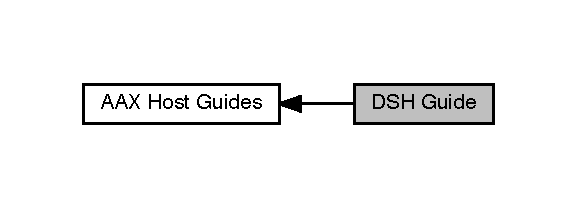
\includegraphics[width=277pt]{a00365}
\end{center}
\end{figure}
